\documentclass[./Spans_of_cospans_II.tex]{subfiles}

%%%%%%%%%%%%%%%%%%%%
%%%%%%%%%%%%%%%%%%%%
%%%%%%%%%%%%%%%%%%%%
%
% BEGIN DOCUMENT
\begin{document}
%
%%%%%%%%%%%%%%%%%%%%
%%%%%%%%%%%%%%%%%%%%
%%%%%%%%%%%%%%%%%%%%

Let $\cat{C}$ be a category with finite limits and colimits.  We claim that there is a bicategory $\cat{Span}(\cat{Cospan}(\cat{C}))$, or $\cat{sc}(\cat{C})$ for short, consisting of
\begin{itemize}
	\item ($0$-cells) $\cat{C}$-objects,
	\item ($1$-cells) $\cat{C}$-cospans, and
	\item ($2$-cells) spans of $\cat{C}$-cospans \emph{up to morphism}.
\end{itemize}
A morphism of spans of $\cat{C}$-cospans is a $\cat{C}$-morphism $\theta$ such that
\[
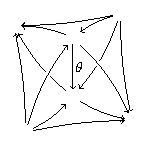
\includegraphics[]{image__scC+Map_of_Spans_of_Cospans.pdf}
\]
commutes. By \emph{up to morphism}, we mean to identify a span of $\cat{C}$-cospans according the equivalence classes generated by the relation $(\theta, \theta')$ if there is a maps of span of $\cat{C}$-cospans $\theta \to \theta'$. An alternative point of view is to say that $\theta \sim \theta'$ if there is a $\tilde{C}$-morphism of type $\iota (\theta) \to \iota (\theta')$ where $\iota \from \cat{C} \hookrightarrow \tilde{C}$ is the inclusion into the groupoid generated by $\cat{C}$. We shall now endeavor to prove that $\cat{sc}(\cat{C})$ is, in fact, a bicategory. 

Fix a pair of $\cat{C}$-objects $x,y$.  Then there is a category $\cat{sc}(\cat{C})(x,y)$ whose objects are the $\cat{C}$-cospans from $x$ to $y$ and the morphisms are spans of $\cat{C}$-cospans up to morphism.  Composition uses pullback as in \eqref{eq:vertical composition}.  Identity functors $I_x \from \cat{1} \to \cat{SCs}(\cat{C})(x,x)$ pick out the $1$-cell $x \to x \gets x$ and the $2$-cell consisting of $x$ and $\cat{C}$-identities on $x$.  

The composition functor $\circ \from \cat{sc}(\cat{C})(y,z) \times \cat{sc}(\cat{C})(x,y) \to \cat{sc}(\cat{C})(x,z)$ acts on morphisms by taking pushouts as in \eqref{eq:horizontal composition}.  
It is straight forward to show that $\circ$ preserves identities.  The composition functor also preserves composition.  To show this, one merely needs to find a $\cat{C}$-morphism as is \eqref{eq:interchange comparison map}, but this certainly exists in a canonical way.  

The associator is defined using the associativity up to isomorphism of pullbacks and pushouts.  The unitors are defined using the fact that the pushout of $x \gets x \to y$ is isomorphic to $y$ when the left leg is the identity.  

The remaining axioms are straightforward to workout. Therefore, $\cat{sc}(\cat{C})$ is a bicategory. In fact, when $\cat{sc}(\cat{C})$ has quite a bit more structure.

%%%%%%%%%%%%%%%%%%%%%%%%%%%%%%%%%%%%%%%%%%%%%%
\subsection{Our bicategory is compact closed}  
%%%%%%%%%%%%%%%%%%%%%%%%%%%%%%%%%%%%%%%%%%%%%%


%%%%%%%%%%%%%%%%%%%%%%%%%%%%%%%%%%%%%%%%%%%%%%%%%%
\subsection{Our bicategory absorbs monoidalness}  
%%%%%%%%%%%%%%%%%%%%%%%%%%%%%%%%%%%%%%%%%%%%%%%%%

Suppose that $\cat{C} \coloneqq (\cat{C}_0, \otimes, I)$ is a symmetric monoidal category.  Using Shulman's work \cite{Shulman}, we will show that $\cat{cs}(\cat{C})$ is a (symmetric, braided) monoidal category. We will not cover the details of Shulman's work here.  The main point we will use, however, is the following theorem.

\begin{thm}[{\cite[{Thm.~1.2}]{Shulman}}]
	\label{thm:Shulmans thm}
	The underlying bicategory of an isofibrant symmetric monoidal double category is symmetric monoidal.  
\end{thm}

Roughly, a \emph{double category} $\DD$ consists of an object category $\DD_\t{ob}$ and arrow category $\DD_\t{ar}$ along with structure functors satisfying certain equations:
\begin{itemize}
	\item $U \from \DD_\t{ob} \to \DD_\t{ar}$ picking out identities,
	\item $S,T \from \DD_\t{ar} \to \DD_\t{ob}$ picking out sources and targets, and
	\item $\odot \from \DD_\t{ar} \times_{\DD_\t{ob}} \DD_\t{ar} \to \DD_\t{ar}$ giving the composition, with the pull back taken over $S$ and $T$.
\end{itemize}
There are also functors realizing associativity plus left and right unity satisfying several properties and coherence axioms.  This can be depicted by
\[
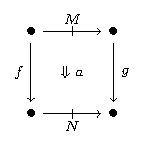
\includegraphics{image__Double_Cat+2Cell_General_Form.pdf}
\]
where the bullets are $\DD_\t{ob}$-objects, $f,g$ are $\DD_\t{ob}$-morphisms, $M,N$ are $\DD_\t{ar}$-objects, and $a$ is a $\DD_\t{ar}$-morphism.  In case $f$ and $g$ are identities, we say that $a$ is \emph{globular}.

There is a lot to unpack from the definition of a symmetric monoidal double category $\DD = (\DD_0,\otimes,I)$, and we will point the interested reader again to Shulman \cite[Def.~2.9]{Shulman}.  The underlying bicategory of $\DD$ is given by
\begin{itemize}
	\item ($0$-cells) $\DD_\t{ob}$-objects,
	\item ($1$-cells) $\DD_\t{ar}$-objects, and
	\item ($2$-cells) globular $\DD_\t{ar}$-morphisms.
\end{itemize}
Also, we say that $\DD$ is \emph{isofibrant} if, for every $\DD_\t{ob}$-morphism $f$, there is a  $\DD_\t{ar}$-object $f'$ together with $\DD_\t{ar}$-morphisms
\[
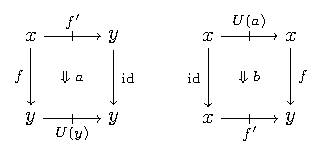
\includegraphics[]{image__Double_Cat+Companion_2Cells.pdf}
\]
that satisfy the equations
\[
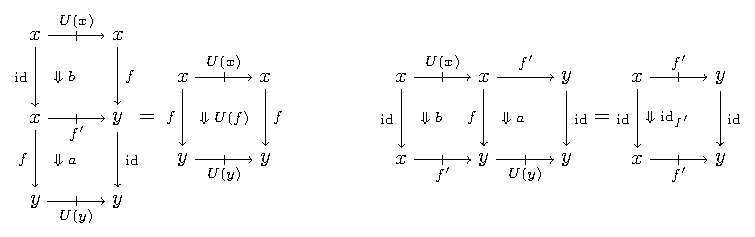
\includegraphics[]{image__Double_Cat+Companion_Equations.pdf}
\]

Now that we know what how to interpret the above theorem, we will construct a double category satisfying the necessary hypothesis. Let $\cat{cs}(\CC)$ be the double category given by the categories 
\[
\cat{cs}(\CC)_\t{ob} \coloneqq \cat{Span}(\cat{C})
\] 
where $\cat{Span}(\cat{C})$ is the $1$-category of spans in $\cat{C}$, and also by
\[
\cat{cs}(\CC)_\t{ar}
\]
whose objects are $\cat{C}$-cospans and morphisms are spans of $\cat{C}$-cospans up to morphism. A morphism in $(\CC)_\t{ar}$ between cospans $x' \to y' \gets z'$ and $x'' \to y'' \gets z''$ is a diagram \todo{arrows wrong direction}
\begin{equation}
\label{eq:2morphism csCC generic}
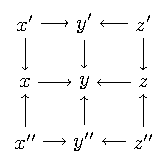
\includegraphics[]{image__csCC+2Morphism_General_Form.pdf}
\end{equation}
in $\cat{C}$ up to morphism, by which we mean the obvious extension of notion of span of cospans up to morphism discussed earlier.  The functor $U \from \cat{cs}(\CC)_\t{ob} \to \cat{cs}(\CC)_\t{ar}$ sends a object to the identity cospan on it and sends a morphism $x \to y \gets z$ to 
\[
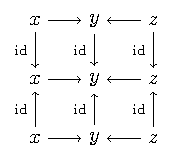
\includegraphics[]{image__csCC+Identity_Functor_U.pdf}
\]
The source functor $S \from \cat{cs}(\CC)_\t{ar} \to \cat{cs}(\CC)_\t{ob}$ sends an object $x \to y \gets z$ to $x$ and a morphism, say \eqref{eq:2morphism csCC generic}, to $x' \to y' \gets z'$.  Define the target functor $T$ similarly.  The composition functor $\odot \from \DD_\t{ar} \times_{\DD_\t{ob}} \DD_\t{ar} \to \DD_\t{ar}$ is more complicated.  We can illustrate its behavior by
\[
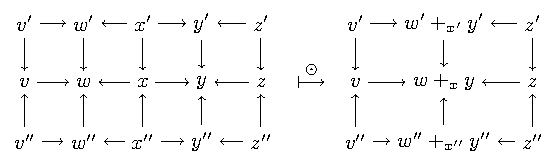
\includegraphics[]{image__csCC+Composition_Functor.pdf}
\]
Then to see whether $\odot$ preserves composition $\circ$, we need to show that 
\begin{equation}
\label{eq:Interchange Law for scCC}
(\alpha \odot \beta) \circ (\alpha' \odot \beta') = (\alpha \circ \beta) \odot (\alpha' \circ \beta'),
\end{equation} 
where
\[
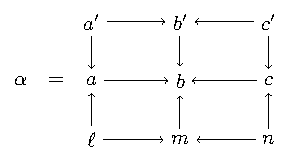
\includegraphics[]{image__scCC+Alpha_2cell.pdf}
\quad
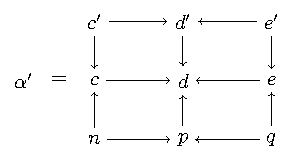
\includegraphics[]{image__scCC+Alpha_Prime_2Cell.pdf}
\]
\[
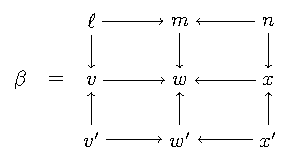
\includegraphics[]{image__scCC+Beta_2Cell.pdf}
\quad
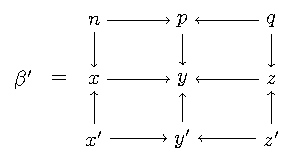
\includegraphics[]{image__scCC+Beta_Prime_2Cell.pdf}
\]
First, we compute the left hand side of \eqref{eq:Interchange Law for scCC}, which corresponds with horizontal composition before vertical composition. \todo{this proof is in your pictures}

And so it's a double category.

Now, let's show that it is isofibrant.  \todo{proof in your pictures.}

Now, let's show that it is symmetric monoidal double category.  
%%%%%%%%%%%%%%%%%%%%%%%%%%%%%%%%%%%%%%%%%%%%%%%%%%%%%%%%%%
\subsection{Symmetric monoidal bicategories} %SM BICATS
\label{subsec.SpansCospansAreSMBicat}
%%%%%%%%%%%%%%%%%%%%%%%%%%%%%%%%%%%%%%%%%%%%%%%%%%%%%%%%%%

\begin{defn}
	\label{def:DblCatMonSpanCsp}
	Let $\cat{C}$ be a finitely complete and cocomplete category. We will define a double category $\dblmonspcsp{C}$ whose objects are the $\cat{C}$-objects, vertical morphisms are given by isomorphism classes of $\cat{C}$-spans with invertible legs, horizontal morphisms are given by $\cat{C}$-cospans, and $2$-morphisms are spans of cospans in $\cat{C}$ making the evident diagram commute (see Figure \ref{fig:2cells}).  
\end{defn}

% DOUBLE CATEGORIES
\begin{lem}
	\label{lem:SpanCospanDoubleCat}
	$\dblmonspcsp{C}$ is a double category.  
\end{lem}

\begin{proof}
	We will denote $\dblmonspcsp{C}$ as $\dblcat{M}$.  Then the object category $\dblcat{M}_0$ is $\cat{Span(C)}$ and the arrow category $\dblcat{M}_1$ is made from $\cat{C}$-cospans and isomorphism classes of $\cat{C}$-spans of cospans.  
	
	The structure functor $U \from \dblcat{M}_0 \to \dblcat{M}_1$ acts on objects by mapping $x$ to the identity cospan on $x$ and acts on morphisms by mapping $y \from x \tospan z$ (whose legs are isomorphisms) to the square
	\[
	\begin{tikzpicture}
	\node (A) at (0,2) {$x$};
	\node (A') at (0,1) {$x$};
	\node (A'') at (0,0) {$x$};
	\node (B) at (1,2) {$y$};
	\node (B') at (1,1) {$y$};
	\node (B'') at (1,0) {$y$};
	\node (C) at (2,2) {$z$};
	\node (C') at (2,1) {$z$};
	\node (C'') at (2,0) {$z$};
	%
	\path[->,font=\scriptsize,>=angle 90]
	% horizontal arrows
	(A) edge node{} (B)
	(A') edge node{} (B')
	(A'') edge node{} (B'')
	(C) edge node{} (B)
	(C') edge node{} (B')
	(C'') edge node{} (B'')
	% vertical arrows
	(A') edge node{} (A)
	(A') edge node{} (A'')
	(B') edge node{} (B)
	(B') edge node{} (B'')
	(C') edge node{} (C)
	(C') edge node{} (C'');
	\end{tikzpicture}
	\]
	filled in with identities and inverses.  The structure functor $S \from \dblcat{M}_1 \to \dblcat{M}_0$ acts on objects by sending $y \from x \tocospan z$ to $x$ and on morphisms by sending a square to the span occupying the left vertical side.  The other functor $T$ is defined similarly.  
	
	The horizontal composition functor $\odot \from \dblcat{M}_1 \times_{\dblcat{M}_0} \dblcat{M}_1 \to \dblcat{M}_1$ acts on objects by composing cospans with pushouts in the usual way.  It acts on morphisms by 
	\[
	\raisebox{-0.5\height}{
		\begin{tikzpicture}
		\node (A) at (0,2) {$a$};
		\node (A') at (0,1) {$a'$};
		\node (A'') at (0,0) {$a''$};
		\node (B) at (1,2) {$b$};
		\node (B') at (1,1) {$b'$};
		\node (B'') at (1,0) {$b''$};
		\node (C) at (2,2) {$c$};
		\node (C') at (2,1) {$c'$};
		\node (C'') at (2,0) {$c''$};
		\node (D) at (3,2) {$d$};
		\node (D') at (3,1) {$d'$};
		\node (D'') at (3,0) {$d''$};
		\node (E) at (4,2) {$e$};
		\node (E') at (4,1) {$e'$};
		\node (E'') at (4,0) {$e''$};
		%
		\path[->,font=\scriptsize,>=angle 90]
		% horizontal arrows
		(A) edge node[above]{} (B)
		(A') edge node[above]{} (B')
		(A'') edge node[above]{} (B'')
		(C) edge node[above]{} (B)
		(C') edge node[above]{} (B')
		(C'') edge node[above]{} (B'')
		(C) edge node[above]{} (D)
		(C') edge node[above]{} (D')
		(C'') edge node[above]{} (D'')
		(E) edge node[above]{} (D)
		(E') edge node[above]{} (D')
		(E'') edge node[above]{} (D'')
		% vertical arrows
		(A') edge node[left]{} (A)
		(A') edge node[left]{} (A'')
		(B') edge node[left]{} (B)
		(B') edge node[left]{} (B'')
		(C') edge node[left]{} (C)
		(C') edge node[left]{} (C'')	
		(D') edge node[left]{} (D)
		(D') edge node[left]{} (D'')
		(E') edge node[left]{} (E)
		(E') edge node[left]{} (E'');
		\end{tikzpicture}
	}
	\quad
	\xmapsto[]{\odot}
	\quad
	\raisebox{-0.5\height}{
		\begin{tikzpicture}
		\node (A) at (0,2) {$a$};
		\node (A') at (0,1) {$a'$};
		\node (A'') at (0,0) {$a''$};
		\node (B) at (1.5,2) {$b+_{c}d$};
		\node (B') at (1.5,1) {$b'+_{c'}d'$};
		\node (B'') at (1.5,0) {$b''+_{c''}d''$};
		\node (C) at (3,2) {$e$};
		\node (C') at (3,1) {$e'$};
		\node (C'') at (3,0) {$e''$};
		%
		\path[->,font=\scriptsize,>=angle 90]
		% horizontal arrows
		(A) edge node[above]{} (B)
		(A') edge node[above]{} (B')
		(A'') edge node[above]{} (B'')
		(C) edge node[above]{} (B)
		(C') edge node[above]{} (B')
		(C'') edge node[above]{} (B'')
		% vertical arrows
		(A') edge node[left]{} (A)
		(A') edge node[left]{} (A'')
		(B') edge node[left]{} (B)
		(B') edge node[left]{} (B'')
		(C') edge node[left]{} (C)
		(C') edge node[left]{} (C'');	
		\end{tikzpicture}
	}
	\]
	This respects indentities, but to see that $\odot$ respects composition, we will wait until the next lemma.  It is straightforward to check that the required equations are satisfied.  
	
	Finally, the associator and unitor natural isomorphisms arise from universal properties.  
\end{proof}

% INTERCHANGE LAW
\begin{lem}
	The assignment $\odot$ from Lemma \ref{lem:SpanCospanDoubleCat} preserves composition. In particular, $\odot$ is a functor.
\end{lem}

\begin{proof}
	Let $\alpha, \alpha^\prime, \beta, \beta^\prime$ be composable $2$-morphisms given by
	\[
	\begin{tikzpicture}
	\node () at (-0.75,1) {$\alpha =$};
	% nodes
	\node (A) at (0,2) {$a$};
	\node (A') at (0,1) {$a'$};
	\node (A'') at (0,0) {$\ell$};
	\node (B) at (1,2) {$b$};
	\node (B') at (1,1) {$b'$};
	\node (B'') at (1,0) {$m$};
	\node (C) at (2,2) {$c$};
	\node (C') at (2,1) {$c'$};
	\node (C'') at (2,0) {$n$};
	%
	\path[->,font=\scriptsize,>=angle 90]
	% horizontal arrows
	(A) edge node[above]{$$} (B)
	(A') edge node[above]{$$} (B')
	(A'') edge node[above]{$$} (B'')
	(C) edge node[above]{$$} (B)
	(C') edge node[above]{$$} (B')
	(C'') edge node[above]{$$} (B'')
	% vertical arrows
	(A') edge node[left]{$\cong$} (A)
	(A') edge node[left]{$\cong$} (A'')
	(B') edge[->] node[left]{} (B)
	(B') edge[->] node[left]{} (B'')
	(C') edge node[left]{$\cong$} (C)
	(C') edge node[left]{$\cong$} (C'');	
	\end{tikzpicture}
	%
	\quad \quad
	%
	\begin{tikzpicture}
	\node () at (-0.75,1) {$\alpha' =$};
	% nodes
	\node (A) at (0,2) {$c$};
	\node (A') at (0,1) {$c'$};
	\node (A'') at (0,0) {$n$};
	\node (B) at (1,2) {$d$};
	\node (B') at (1,1) {$d'$};
	\node (B'') at (1,0) {$p$};
	\node (C) at (2,2) {$e$};
	\node (C') at (2,1) {$e'$};
	\node (C'') at (2,0) {$q$};
	%
	\path[->,font=\scriptsize,>=angle 90]
	% horizontal arrows
	(A) edge node[above]{$$} (B)
	(A') edge node[above]{$$} (B')
	(A'') edge node[above]{$$} (B'')
	(C) edge node[above]{$$} (B)
	(C') edge node[above]{$$} (B')
	(C'') edge node[above]{$$} (B'')
	% vertical arrows
	(A') edge node[left]{$\cong$} (A)
	(A') edge node[left]{$\cong$} (A'')
	(B') edge[->] node[left]{} (B)
	(B') edge[->] node[left]{} (B'')
	(C') edge node[left]{$\cong$} (C)
	(C') edge node[left]{$\cong$} (C'');	
	\end{tikzpicture}
	\]
	%
	%
	\[
	\begin{tikzpicture}
	\node () at (-0.75,1) {$\beta =$};
	% nodes
	\node (A) at (0,2) {$\ell$};
	\node (A') at (0,1) {$v'$};
	\node (A'') at (0,0) {$v$};
	\node (B) at (1,2) {$m$};
	\node (B') at (1,1) {$w'$};
	\node (B'') at (1,0) {$w$};
	\node (C) at (2,2) {$n$};
	\node (C') at (2,1) {$x'$};
	\node (C'') at (2,0) {$x$};
	%
	\path[->,font=\scriptsize,>=angle 90]
	% horizontal arrows
	(A) edge node[above]{$$} (B)
	(A') edge node[above]{$$} (B')
	(A'') edge node[above]{$$} (B'')
	(C) edge node[above]{$$} (B)
	(C') edge node[above]{$$} (B')
	(C'') edge node[above]{$$} (B'')
	% vertical arrows
	(A') edge node[left]{$\cong$} (A)
	(A') edge node[left]{$\cong$} (A'')
	(B') edge[->] node[left]{} (B)
	(B') edge[->] node[left]{} (B'')
	(C') edge node[left]{$\cong$} (C)
	(C') edge node[left]{$\cong$} (C'');	
	\end{tikzpicture}
	\quad \quad
	%
	%
	\begin{tikzpicture}
	\node () at (-0.75,1) {$\beta' =$};
	% nodes
	\node (A) at (0,2) {$n$};
	\node (A') at (0,1) {$x'$};
	\node (A'') at (0,0) {$x$};
	\node (B) at (1,2) {$p$};
	\node (B') at (1,1) {$y'$};
	\node (B'') at (1,0) {$y$};
	\node (C) at (2,2) {$q$};
	\node (C') at (2,1) {$z'$};
	\node (C'') at (2,0) {$z$};
	%
	\path[->,font=\scriptsize,>=angle 90]
	% horizontal arrows
	(A) edge node[above]{$$} (B)
	(A') edge node[above]{$$} (B')
	(A'') edge node[above]{$$} (B'')
	(C) edge node[above]{$$} (B)
	(C') edge node[above]{$$} (B')
	(C'') edge node[above]{$$} (B'')
	% vertical arrows
	(A') edge node[left]{$\cong$} (A)
	(A') edge node[left]{$\cong$} (A'')
	(B') edge[->] node[left]{} (B)
	(B') edge[->] node[left]{} (B'')
	(C') edge node[left]{$\cong$} (C)
	(C') edge node[left]{$\cong$} (C'');	
	\end{tikzpicture}
	\]
	Our goal is to show that
	\begin{equation}
	\label{eq:InterchangeCspSpan}
	(\alpha \odot \alpha') \circ (\beta \odot \beta')
	=
	(\alpha \circ \beta) \odot (\alpha' \circ \beta').
	\end{equation}
	The left hand side of this equation corresponds to horizontal composition before vertical composition, while the right hand side reverses the order.
	
	First, we will compute the left hand side of \eqref{eq:InterchangeCspSpan}. Composing horizontally we get that $\alpha \odot \alpha'$ and $\beta \odot \beta'$ are, respectively,
	\[
	\begin{tikzpicture}
	\node (A) at (1,1) {$a$};
	\node (A') at (1,0) {$a'$};
	\node (A'') at (1,-1) {$\ell$};
	\node (B) at (3,1) {$b+_{c}d$};
	\node (B') at (3,0) {$b'+_{c'}d'$};
	\node (B'') at (3,-1) {$m+_{n}p$};
	\node (C) at (5,1) {$e$};
	\node (C') at (5,0) {$e'$};
	\node (C'') at (5,-1) {$q$};
	%
	\path[->,font=\scriptsize,>=angle 90]
	% horizontal arrows
	(A) edge node[above]{$$} (B)
	(A') edge node[above]{$$} (B')
	(A'') edge node[above]{$$} (B'')
	(C) edge node[above]{$$} (B)
	(C') edge node[above]{$$} (B')
	(C'') edge node[above]{$$} (B'')
	% vertical arrows
	(A') edge node[left]{$\cong$} (A)
	(A') edge node[left]{$\cong$} (A'')
	(B') edge[->] node[left]{} (B)
	(B') edge[->] node[left]{} (B'')
	(C') edge node[left]{$\cong$} (C)
	(C') edge node[left]{$\cong$} (C'');	
	\end{tikzpicture}
	%
	\quad \quad
	%
	\begin{tikzpicture}
	\node (A) at (1,1) {$\ell$};
	\node (A') at (1,0) {$v'$};
	\node (A'') at (1,-1) {$v$};
	\node (B) at (3,1) {$m+_{n}p$};
	\node (B') at (3,0) {$w'+_{x'}y'$};
	\node (B'') at (3,-1) {$w+_{x}y$};
	\node (C) at (5,1) {$q$};
	\node (C') at (5,0) {$z'$};
	\node (C'') at (5,-1) {$z$};
	%
	\path[->,font=\scriptsize,>=angle 90]
	% horizontal arrows
	(A) edge node[above]{$$} (B)
	(A') edge node[above]{$$} (B')
	(A'') edge node[above]{$$} (B'')
	(C) edge node[above]{$$} (B)
	(C') edge node[above]{$$} (B')
	(C'') edge node[above]{$$} (B'')
	% vertical arrows
	(A') edge node[left]{$\cong$} (A)
	(A') edge node[left]{$\cong$} (A'')
	(B') edge[->] node[left]{} (B)
	(B') edge[->] node[left]{} (B'')
	(C') edge node[left]{$\cong$} (C)
	(C') edge node[left]{$\cong$} (C'');	
	\end{tikzpicture}
	\]
	Next, composing $\alpha \odot \alpha^\prime$ and $\beta \odot \beta^\prime$ vertically, we get that $(\alpha \odot \alpha^\prime) \circ (\beta \odot \beta^\prime)$ is equal to
	\begin{equation}
	\label{diag:IntrchngHorVertCspSpan}
	\raisebox{-0.5\height}{
		\begin{tikzpicture}
		\node (A) at (1,1) {$a$};
		\node (A') at (1,0) {$a'\times_{\ell}v'$};
		\node (A'') at (1,-1) {$v$};
		\node (B) at (5,1) {$b+_{d}d$};
		\node (B') at (5,0) {$(b'+_{c'}d') \times_{(m+_{n}p)} (w'+_{x'}y')$};
		\node (B'') at (5,-1) {$w+_{x}y$};
		\node (C) at (9,1) {$e$};
		\node (C') at (9,0) {$e' +_{q}z'$};
		\node (C'') at (9,-1) {$z$};
		%
		\path[->,font=\scriptsize,>=angle 90]
		% horizontal arrows
		(A) edge node[above]{$$} (B)
		(A') edge node[above]{$$} (B')
		(A'') edge node[above]{$$} (B'')
		(C) edge node[above]{$$} (B)
		(C') edge node[above]{$$} (B')
		(C'') edge node[above]{$$} (B'')
		% vertical arrows
		(A') edge node[left]{$\cong$} (A)
		(A') edge node[left]{$\cong$} (A'')
		(B') edge[->] node[left]{} (B)
		(B') edge[->] node[left]{} (B'')
		(C') edge node[left]{$\cong$} (C)
		(C') edge node[left]{$\cong$} (C'');	
		\end{tikzpicture}
	}
	\end{equation}
	
	Now solving for the right hand side of \eqref{eq:InterchangeCspSpan}, we first obtain that $\alpha \circ \beta$ and $\alpha' \circ \beta'$ are, respectively,
	\[
	\begin{tikzpicture}
	\node (A) at (1,1) {$a$};
	\node (A') at (1,0) {$a' \times_{\ell}v'$};
	\node (A'') at (1,-1) {$v$};
	\node (B) at (3,1) {$b$};
	\node (B') at (3,0) {$b' \times_{m}w'$};
	\node (B'') at (3,-1) {$w$};
	\node (C) at (5,1) {$c$};
	\node (C') at (5,0) {$c' \times_{n}x'$};
	\node (C'') at (5,-1) {$x$};
	%
	\path[->,font=\scriptsize,>=angle 90]
	% horizontal arrows
	(A) edge node[above]{$$} (B)
	(A') edge node[above]{$$} (B')
	(A'') edge node[above]{$$} (B'')
	(C) edge node[above]{$$} (B)
	(C') edge node[above]{$$} (B')
	(C'') edge node[above]{$$} (B'')
	% vertical arrows
	(A') edge node[left]{$\cong$} (A)
	(A') edge node[left]{$\cong$} (A'')
	(B') edge[->] node[left]{} (B)
	(B') edge[->] node[left]{} (B'')
	(C') edge node[left]{$\cong$} (C)
	(C') edge node[left]{$\cong$} (C'');	
	\end{tikzpicture}
	%
	\quad \quad 
	%
	\begin{tikzpicture}
	\node (A) at (1,1) {$c$};
	\node (A') at (1,0) {$c' \times_{n}x'$};
	\node (A'') at (1,-1) {$x$};
	\node (B) at (3,1) {$d$};
	\node (B') at (3,0) {$d' \times_{p}y'$};
	\node (B'') at (3,-1) {$y$};
	\node (C) at (5,1) {$e$};
	\node (C') at (5,0) {$e' \times_{q}z'$};
	\node (C'') at (5,-1) {$z$};
	%
	\path[->,font=\scriptsize,>=angle 90]
	% horizontal arrows
	(A) edge node[above]{$$} (B)
	(A') edge node[above]{$$} (B')
	(A'') edge node[above]{$$} (B'')
	(C) edge node[above]{$$} (B)
	(C') edge node[above]{$$} (B')
	(C'') edge node[above]{$$} (B'')
	% vertical arrows
	(A') edge node[left]{$\cong$} (A)
	(A') edge node[left]{$\cong$} (A'')
	(B') edge[->] node[left]{} (B)
	(B') edge[->] node[left]{} (B'')
	(C') edge node[left]{$\cong$} (C)
	(C') edge node[left]{$\cong$} (C'');	
	\end{tikzpicture}
	\]
	Now composing these vertically, we get that $(\alpha \circ \beta) \odot (\alpha^\prime \circ \beta^\prime)$ equals
	\begin{equation}
	\label{diag:IntrchngVertHorCspSpan}
	\raisebox{-0.5\height}{
		\begin{tikzpicture}
		\node (A) at (1,1) {$a$};
		\node (A') at (1,0) {$a' \times_{\ell}v'$};
		\node (A'') at (1,-1) {$v$};
		\node (B) at (5,1) {$b +_{c}d$};
		\node (B') at (5,0) {$(b'\times_{m}w')+_{(c'\times_{n}x')}(d'\times_{p}y')$};
		\node (B'') at (5,-1) {$w+_{x}y$};
		\node (C) at (9,1) {$e$};
		\node (C') at (9,0) {$e' \times_{q}z'$};
		\node (C'') at (9,-1) {$z$};
		%
		\path[->,font=\scriptsize,>=angle 90]
		% horizontal arrows
		(A) edge node[above]{$$} (B)
		(A') edge node[above]{$$} (B')
		(A'') edge node[above]{$$} (B'')
		(C) edge node[above]{$$} (B)
		(C') edge node[above]{$$} (B')
		(C'') edge node[above]{$$} (B'')
		% vertical arrows
		(A') edge node[left]{$\cong$} (A)
		(A') edge node[left]{$\cong$} (A'')
		(B') edge[->] node[left]{} (B)
		(B') edge[->] node[left]{} (B'')
		(C') edge node[left]{$\cong$} (C)
		(C') edge node[left]{$\cong$} (C'');	
		\end{tikzpicture}
	}
	\end{equation}
	
	Now, we need to show that \eqref{diag:IntrchngHorVertCspSpan} is equal to \eqref{diag:IntrchngVertHorCspSpan} as $2$-morphisms.  Note that the diagrams only differ in the middle.  Thus the proof of the interchange law is the canonical map
	\[
	(b'+_{c'}d') \times_{(m+_{n}p)} (w'+_{x'}y')
	\to 
	(b' \times_{m}w')+_{(c'\times_{n}x')}(d'\times_{p}y')
	\]
\end{proof}


% DOUBLE CATEGORIES ARE SYMMETRIC MONOIDAL
\begin{lem}
	\label{lem:SpanCospanSM}
	$\dblmonspcsp{C}$ is a symmetric monoidal double category.  
\end{lem}

\begin{proof}
	Let us first show that the object $\dblcat{M}_0$ and arrow $\dblcat{M}_1$ categories are symmetric monoidal.  Note that $\dblcat{M}_0$ is the largest groupoid contained in $\spcsp{C}$. We can give it monoidal structure via the already present $\otimes$ and $I$ in $\cat{C}$ on objects and
	\[
	(b \from a \tospan c) \otimes (b' \from a' \tospan c')
	=
	(b\otimes b' \from a\otimes a' \tocospan c\otimes c')
	\]
	on morphisms.  Universal properties provide the associator and unitors as well as the coherence axioms. This monoidal structure is clearly symmetric.
	
	Note that $\dblcat{M}_1$ is the category of $\cat{C}$-cospans and morphism classes of $\cat{C}$-spans of cospans  causing the evident diagrams to commute (see Figure \ref{fig:2cells}).  We obtain a symmetric monoidal structure on the objects via 
	\[
	(b \from a \tocospan c) \otimes (b' \from a' \tocospan c')
	=
	(b\otimes b' \from a\otimes a' \tocospan c\otimes c')
	\]
	and on the morphisms by
	\[
	\raisebox{-0.5\height}{
		\begin{tikzpicture}
		\node (A) at (0,2) {$\bullet$};
		\node (A') at (0,1) {$\bullet$};
		\node (A'') at (0,0) {$\bullet$};
		\node (B) at (1,2) {$\bullet$};
		\node (B') at (1,1) {$\bullet$};
		\node (B'') at (1,0) {$\bullet$};
		\node (C) at (2,2) {$\bullet$};
		\node (C') at (2,1) {$\bullet$};
		\node (C'') at (2,0) {$\bullet$};
		%
		\path[->,font=\scriptsize,>=angle 90]
		% horizontal arrows
		(A) edge node[above]{} (B)
		(A') edge node[above]{} (B')
		(A'') edge node[above]{} (B'')
		(C) edge node[above]{} (B)
		(C') edge node[above]{} (B')
		(C'') edge node[above]{} (B'')
		% vertical arrows
		(A') edge node[left]{} (A)
		(A') edge node[left]{} (A'')
		(B') edge[->] node[left]{} (B)
		(B') edge[->] node[left]{} (B'')
		(C') edge node[left]{} (C)
		(C') edge node[left]{} (C'');	
		\end{tikzpicture}
	}
	%
	\quad \otimes \quad
	%
	\raisebox{-0.5\height}{
		\begin{tikzpicture}
		\node (A) at (0,2) {$\ast$};
		\node (A') at (0,1) {$\ast$};
		\node (A'') at (0,0) {$\ast$};
		\node (B) at (1,2) {$\ast$};
		\node (B') at (1,1) {$\ast$};
		\node (B'') at (1,0) {$\ast$};
		\node (C) at (2,2) {$\ast$};
		\node (C') at (2,1) {$\ast$};
		\node (C'') at (2,0) {$\ast$};
		%
		\path[->,font=\scriptsize,>=angle 90]
		% horizontal arrows
		(A) edge node[above]{} (B)
		(A') edge node[above]{} (B')
		(A'') edge node[above]{} (B'')
		(C) edge node[above]{} (B)
		(C') edge node[above]{} (B')
		(C'') edge node[above]{} (B'')
		% vertical arrows
		(A') edge node[left]{} (A)
		(A') edge node[left]{} (A'')
		(B') edge[->] node[left]{} (B)
		(B') edge[->] node[left]{} (B'')
		(C') edge node[left]{} (C)
		(C') edge node[left]{} (C'');	
		\end{tikzpicture}
	}
	%
	\quad = \quad
	%
	\raisebox{-0.5\height}{
		\begin{tikzpicture}
		\node (A) at (0,2) {$\bullet\otimes \ast$};
		\node (A') at (0,1) {$\bullet\otimes \ast$};
		\node (A'') at (0,0) {$\bullet\otimes \ast$};
		\node (B) at (1.5,2) {$\bullet\otimes \ast$};
		\node (B') at (1.5,1) {$\bullet\otimes \ast$};
		\node (B'') at (1.5,0) {$\bullet\otimes \ast$};
		\node (C) at (3,2) {$\bullet\otimes \ast$};
		\node (C') at (3,1) {$\bullet\otimes \ast$};
		\node (C'') at (3,0) {$\bullet\otimes \ast$};
		%
		\path[->,font=\scriptsize,>=angle 90]
		% horizontal arrows
		(A) edge node[above]{} (B)
		(A') edge node[above]{} (B')
		(A'') edge node[above]{} (B'')
		(C) edge node[above]{} (B)
		(C') edge node[above]{} (B')
		(C'') edge node[above]{} (B'')
		% vertical arrows
		(A') edge node[left]{} (A)
		(A') edge node[left]{} (A'')
		(B') edge[>->] node[left]{} (B)
		(B') edge[>->] node[left]{} (B'')
		(C') edge node[left]{} (C)
		(C') edge node[left]{} (C'');	
		\end{tikzpicture}
	}
	\]
	Again, universal properties provide the associator, unitors, and the coherence axioms.  Hence both $\dblcat{M}_0$ and $\dblcat{M}_1$ are symmetric monoidal categories.
	
	Because $\dblmonspcsp{C}$ has the same horizontal morphisms as $\dblcspcsp{C}$, we can use the same globular isomorphisms for each case but turning vertically aligned spans into cospans by using inverses.  It follows that the required diagrams will commute.
\end{proof}

% DOUBLE CATEGORIES ARE ISOFIBRANT
\begin{lem}
	\label{lem:SpanCospanIsofibrant}
	$\dblmonspcsp{T}$ is isofibrant.  
\end{lem}

\begin{proof}
	Take a vertical morphism $f = (b \from a \tospan c)$ whose legs are isomorphisms. Its companion $\widehat{f} = (b \from a \tocospan c)$ where the legs are given by the inverses of the legs of $f$, along with the $2$-morphisms
	\[
	\raisebox{-0.5\height}{
		\begin{tikzpicture}
		\node (A) at (0,2) {$a$};
		\node (A') at (0,1) {$b$};
		\node (A'') at (0,0) {$c$};
		\node (B) at (1,2) {$b$};
		\node (B') at (1,1) {$c$};
		\node (B'') at (1,0) {$c$};
		\node (C) at (2,2) {$c$};
		\node (C') at (2,1) {$c$};
		\node (C'') at (2,0) {$c$};
		%
		\path[->,font=\scriptsize,>=angle 90]
		% horizontal arrows
		(A) edge node[above]{} (B)
		(A') edge node[above]{} (B')
		(A'') edge node[above]{} (B'')
		(C) edge node[above]{} (B)
		(C') edge node[above]{} (B')
		(C'') edge node[above]{} (B'')
		% vertical arrows
		(A') edge node[left]{} (A)
		(A') edge node[left]{} (A'')
		(B') edge node[left]{} (B)
		(B') edge node[left]{} (B'')
		(C') edge node[left]{} (C)
		(C') edge node[left]{} (C'');
		\end{tikzpicture}
	}
	%
	\t{ and }
	%
	\raisebox{-0.5\height}{
		\begin{tikzpicture}
		\node (A) at (0,2) {$a$};
		\node (A') at (0,1) {$a$};
		\node (A'') at (0,0) {$a$};
		\node (B) at (1,2) {$a$};
		\node (B') at (1,1) {$a$};
		\node (B'') at (1,0) {$b$};
		\node (C) at (2,2) {$a$};
		\node (C') at (2,1) {$b$};
		\node (C'') at (2,0) {$c$};
		%
		\path[->,font=\scriptsize,>=angle 90]
		% horizontal arrows
		(A) edge node[above]{} (B)
		(A') edge node[above]{} (B')
		(A'') edge node[above]{} (B'')
		(C) edge node[above]{} (B)
		(C') edge node[above]{} (B')
		(C'') edge node[above]{} (B'')
		% vertical arrows
		(A') edge node[left]{} (A)
		(A') edge node[left]{} (A'')
		(B') edge node[left]{} (B)
		(B') edge node[left]{} (B'')
		(C') edge node[left]{} (C)
		(C') edge node[left]{} (C'');
		\end{tikzpicture}
	}
	\]
	The conjoint for $f$ is given by $\check{f} = \widehat{f}^{\text{op}}$.
\end{proof}

% BICATEEGORIES
\begin{thm}
	\label{thm:SpansCospasAreSMBicat}
	$\spcsp{C}$ is a symmetric monoidal bicategory.
\end{thm}

\begin{proof}
	Apply Theorem \ref{thm:DoubleGivesBi}.
\end{proof}

%%%%%%%%%%%%%%%%%%%%%%%%%%%%%%%%%%%%%%%%%%%%%%%%%%%%%%%%%%
\subsection{Compact closed} % COMPACT CLOSED 
\label{subsec.SpansCospansAreCCBicats}
%%%%%%%%%%%%%%%%%%%%%%%%%%%%%%%%%%%%%%%%%%%%%%%%%%%%%%%%%%

\begin{thm}
	\label{thm:SpansCospansAreCCBicat}
	$\spcsp{C}$ is compact closed.
\end{thm}

\begin{proof}
	To begin, we will show that objects are self dual. Take an object $X$.  Define the evaluation morphism $e \from X \otimes X \tocospan I$ and coevaluation morphism $c \from I \tocospan X\otimes X$ as follows:
	\[
	e = (X\otimes X \xto{\nabla} X \gets I), \quad \quad 
	c = (I \to X \xleftarrow{\nabla} X \otimes X).
	\]
	Next we define the cusp isomorphisms, $\alpha$ and $\beta$.
	Note that $\alpha$ is a $2$-morphism whose domain is the composite morphism
	\[
	X \xto{\ell}
	X\otimes X \xleftarrow{X\otimes \nabla}
	X\otimes X\otimes X \xto{\nabla \otimes X}
	X\otimes X \xleftarrow{r}
	X
	\]
	and codomain is the identity cospan on $X$.  Use Lemma \ref{lem:PushoutDiagram} and the fact that $\nabla\otimes X = \ell \circ \nabla$ and $X \otimes  \nabla = r \circ \nabla$ to see that the composite is the identity cospan on $X$.  The codomain of $\beta$ is also the identity cospan on $X$, which is obtained as the composite morphism
	\[
	X \xto{r}
	X\otimes X \xleftarrow{\nabla\otimes X}
	X\otimes X\otimes X \xto{X\otimes \nabla}
	X\otimes X \xleftarrow{\ell}
	X
	\]
	Take $\alpha$ and $\beta$, each, to be the identity $2$-morphism on $X$. Thus we have a dual pair $(X,X,e,c,\alpha,\beta)$. By Theorem \ref{thm:StrictingDualPairs}, we know there is a cusp isomorphism $\beta'$ such that $(X,X,e,c,\alpha,\beta')$ is a coherent dual pair.  
\end{proof}


%%%%%%%%%%%%%%%%%%%%
%%%%%%%%%%%%%%%%%%%%
%%%%%%%%%%%%%%%%%%%%
%
% END DOCUMENT
\end{document}
%
%%%%%%%%%%%%%%%%%%%%
%%%%%%%%%%%%%%%%%%%%
%%%%%%%%%%%%%%%%%%%%
